
\documentclass[margin=10pt]{report}
\usepackage{pgfplots}
\usepgfplotslibrary{statistics}
\begin{document}
        
    %\pgfplotsset{height=\bighistheight}
    \centering
    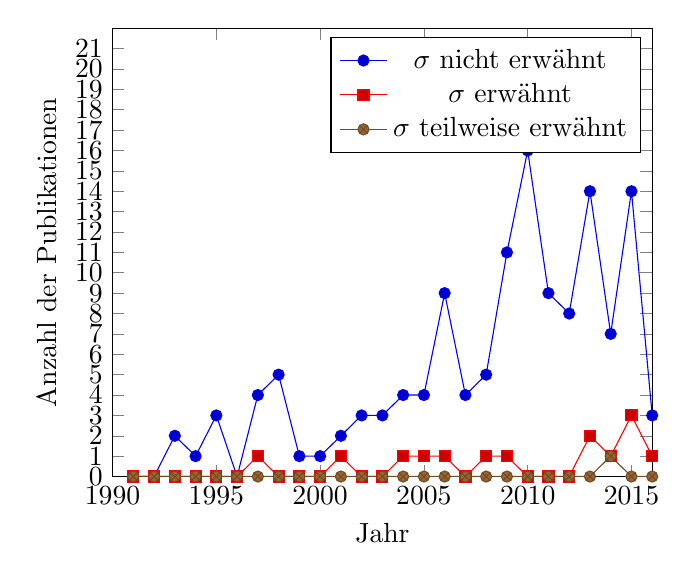
\begin{tikzpicture}
        \begin{axis}[
        ymin=0,
        ymax=22,
        %xtick = 1,
        bar shift=0pt,
        %enlarge x limits=0.10,
        xtick = {1990, 1995, 2000, 2005, 2010, 2015},
        xmin = 1990,
        xmax = 2016,
        ytick = {0, ..., 21},
        cycle list name=auto,
        %every axis plot/.append style={ybar interval, opacity=0.75,fill,draw=black,no markers},
        ylabel={Anzahl der Publikationen},
        xlabel=Jahr,
        x tick label style={/pgf/number format/.cd, set thousands separator={}},
        legend entries={$\sigma$ nicht erwähnt\\$\sigma$ erwähnt\\$\sigma$ teilweise erwähnt\\}
        ]
            \addplot coordinates {(1991, 0) (1992, 0) (1993, 2) (1994, 1) (1995, 3) (1996, 0) (1997, 4) (1998, 5) (1999, 1) (2000, 1) (2001, 2) (2002, 3) (2003, 3) (2004, 4) (2005, 4) (2006, 9) (2007, 4) (2008, 5) (2009, 11) (2010, 16) (2011, 9) (2012, 8) (2013, 14) (2014, 7) (2015, 14) (2016, 3)};
            \addplot coordinates {(1991, 0) (1992, 0) (1993, 0) (1994, 0) (1995, 0) (1996, 0) (1997, 1) (1998, 0) (1999, 0) (2000, 0) (2001, 1) (2002, 0) (2003, 0) (2004, 1) (2005, 1) (2006, 1) (2007, 0) (2008, 1) (2009, 1) (2010, 0) (2011, 0) (2012, 0) (2013, 2) (2014, 1) (2015, 3) (2016, 1)};
            \addplot coordinates {(1991, 0) (1992, 0) (1993, 0) (1994, 0) (1995, 0) (1996, 0) (1997, 0) (1998, 0) (1999, 0) (2000, 0) (2001, 0) (2002, 0) (2003, 0) (2004, 0) (2005, 0) (2006, 0) (2007, 0) (2008, 0) (2009, 0) (2010, 0) (2011, 0) (2012, 0) (2013, 0) (2014, 1) (2015, 0) (2016, 0)};
        \end{axis}
    \end{tikzpicture}

    std = 14 und   9\%, both = 1 und   1\%, no std = 133 und  90\%


    
    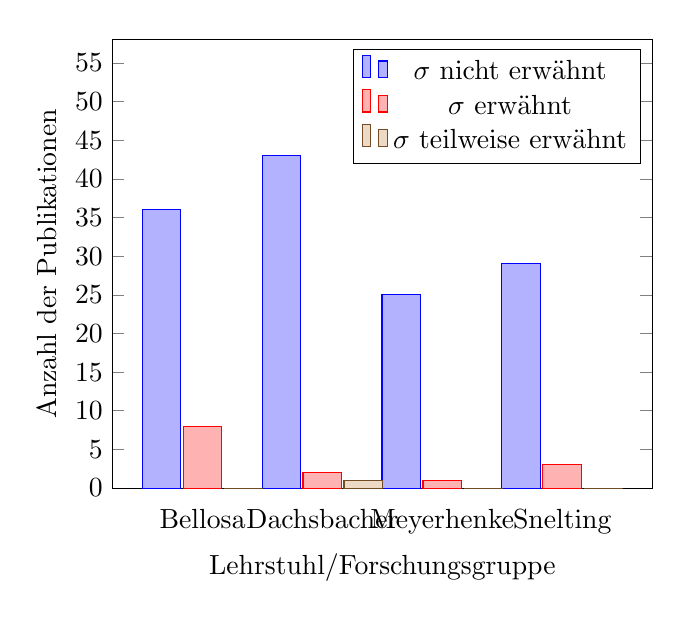
\begin{tikzpicture}
        \begin{axis}[
        major x tick style = transparent,
        ybar=2*\pgflinewidth,
        bar width=14pt,
        ylabel = {Anzahl der Publikationen},
        symbolic x coords={Bellosa,Dachsbacher,Meyerhenke,Snelting},
        xlabel = {Lehrstuhl/Forschungsgruppe},
        xtick = data,
        scaled y ticks = false,
        enlarge x limits=0.25,
        ymin=0,
        ymax=58,
        ytick = {0, 5, ..., 57},
        cycle list name=auto,
        legend entries={$\sigma$ nicht erwähnt\\$\sigma$ erwähnt\\$\sigma$ teilweise erwähnt\\}
        ]
            \addplot coordinates {(Bellosa, 36) (Dachsbacher, 43) (Meyerhenke, 25) (Snelting, 29)};
            \addplot coordinates {(Bellosa, 8) (Dachsbacher, 2) (Meyerhenke, 1) (Snelting, 3)};
            \addplot coordinates {(Bellosa, 0) (Dachsbacher, 1) (Meyerhenke, 0) (Snelting, 0)};
        \end{axis}
    \end{tikzpicture}

    std = 14, both = 1, no std = 133


    \section{meyerhenke}

    %\pgfplotsset{height=\bighistheight}
    \centering
    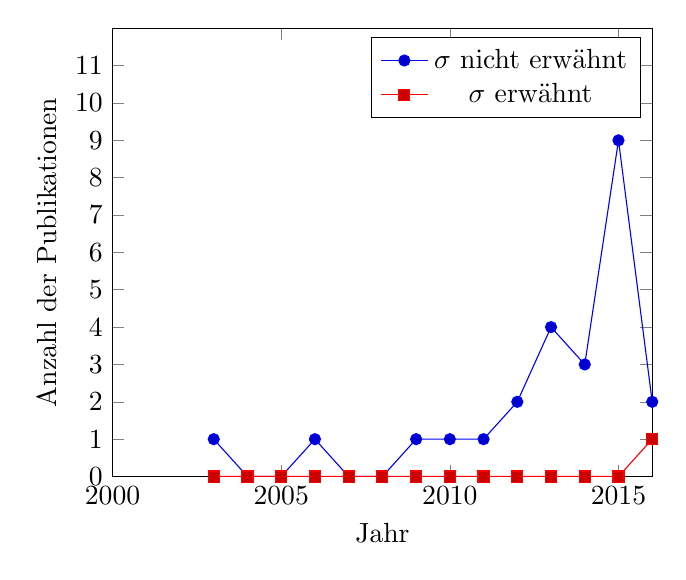
\begin{tikzpicture}
        \begin{axis}[
        ymin=0,
        ymax=12,
        %xtick = 1,
        bar shift=0pt,
        %enlarge x limits=0.10,
        xtick = {2000, 2005, 2010, 2015},
        xmin = 2000,
        xmax = 2016,
        ytick = {0, ..., 11},
        cycle list name=auto,
        %every axis plot/.append style={ybar interval, opacity=0.75,fill,draw=black,no markers},
        ylabel={Anzahl der Publikationen},
        xlabel=Jahr,
        x tick label style={/pgf/number format/.cd, set thousands separator={}},
        legend entries={$\sigma$ nicht erwähnt\\$\sigma$ erwähnt\\}
        ]
            \addplot coordinates {(2003, 1) (2004, 0) (2005, 0) (2006, 1) (2007, 0) (2008, 0) (2009, 1) (2010, 1) (2011, 1) (2012, 2) (2013, 4) (2014, 3) (2015, 9) (2016, 2)};
            \addplot coordinates {(2003, 0) (2004, 0) (2005, 0) (2006, 0) (2007, 0) (2008, 0) (2009, 0) (2010, 0) (2011, 0) (2012, 0) (2013, 0) (2014, 0) (2015, 0) (2016, 1)};
        \end{axis}
    \end{tikzpicture}

    std = 1 und   4\%, both = 0 und   0\%, no std = 25 und  96\%


    \section{snelting}

    %\pgfplotsset{height=\bighistheight}
    \centering
    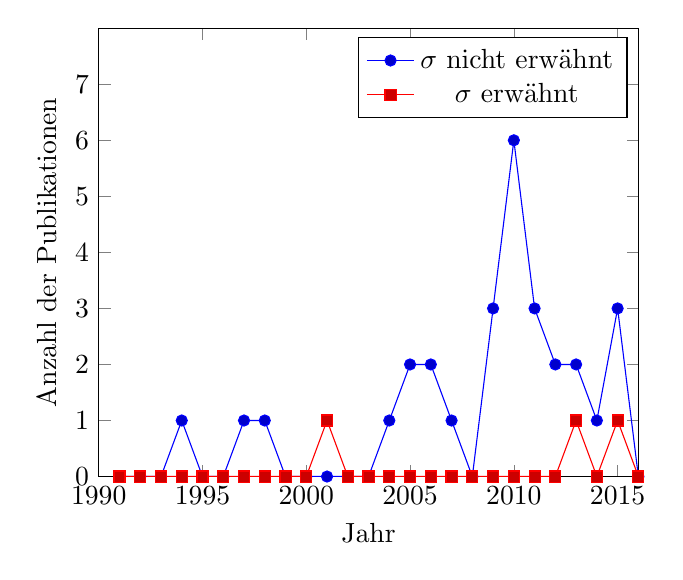
\begin{tikzpicture}
        \begin{axis}[
        ymin=0,
        ymax=8,
        %xtick = 1,
        bar shift=0pt,
        %enlarge x limits=0.10,
        xtick = {1990, 1995, 2000, 2005, 2010, 2015},
        xmin = 1990,
        xmax = 2016,
        ytick = {0, ..., 7},
        cycle list name=auto,
        %every axis plot/.append style={ybar interval, opacity=0.75,fill,draw=black,no markers},
        ylabel={Anzahl der Publikationen},
        xlabel=Jahr,
        x tick label style={/pgf/number format/.cd, set thousands separator={}},
        legend entries={$\sigma$ nicht erwähnt\\$\sigma$ erwähnt\\}
        ]
            \addplot coordinates {(1991, 0) (1992, 0) (1993, 0) (1994, 1) (1995, 0) (1996, 0) (1997, 1) (1998, 1) (1999, 0) (2000, 0) (2001, 0) (2002, 0) (2003, 0) (2004, 1) (2005, 2) (2006, 2) (2007, 1) (2008, 0) (2009, 3) (2010, 6) (2011, 3) (2012, 2) (2013, 2) (2014, 1) (2015, 3) (2016, 0)};
            \addplot coordinates {(1991, 0) (1992, 0) (1993, 0) (1994, 0) (1995, 0) (1996, 0) (1997, 0) (1998, 0) (1999, 0) (2000, 0) (2001, 1) (2002, 0) (2003, 0) (2004, 0) (2005, 0) (2006, 0) (2007, 0) (2008, 0) (2009, 0) (2010, 0) (2011, 0) (2012, 0) (2013, 1) (2014, 0) (2015, 1) (2016, 0)};
        \end{axis}
    \end{tikzpicture}

    std = 3 und   9\%, both = 0 und   0\%, no std = 29 und  91\%


    \section{bellossa}

    %\pgfplotsset{height=\bighistheight}
    \centering
    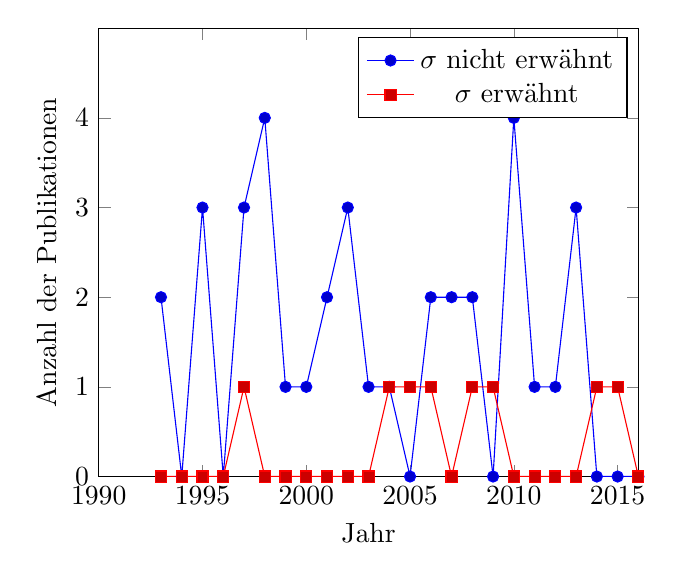
\begin{tikzpicture}
        \begin{axis}[
        ymin=0,
        ymax=5,
        %xtick = 1,
        bar shift=0pt,
        %enlarge x limits=0.10,
        xtick = {1990, 1995, 2000, 2005, 2010, 2015},
        xmin = 1990,
        xmax = 2016,
        ytick = {0, ..., 4},
        cycle list name=auto,
        %every axis plot/.append style={ybar interval, opacity=0.75,fill,draw=black,no markers},
        ylabel={Anzahl der Publikationen},
        xlabel=Jahr,
        x tick label style={/pgf/number format/.cd, set thousands separator={}},
        legend entries={$\sigma$ nicht erwähnt\\$\sigma$ erwähnt\\}
        ]
            \addplot coordinates {(1993, 2) (1994, 0) (1995, 3) (1996, 0) (1997, 3) (1998, 4) (1999, 1) (2000, 1) (2001, 2) (2002, 3) (2003, 1) (2004, 1) (2005, 0) (2006, 2) (2007, 2) (2008, 2) (2009, 0) (2010, 4) (2011, 1) (2012, 1) (2013, 3) (2014, 0) (2015, 0) (2016, 0)};
            \addplot coordinates {(1993, 0) (1994, 0) (1995, 0) (1996, 0) (1997, 1) (1998, 0) (1999, 0) (2000, 0) (2001, 0) (2002, 0) (2003, 0) (2004, 1) (2005, 1) (2006, 1) (2007, 0) (2008, 1) (2009, 1) (2010, 0) (2011, 0) (2012, 0) (2013, 0) (2014, 1) (2015, 1) (2016, 0)};
        \end{axis}
    \end{tikzpicture}

    std = 8 und  18\%, both = 0 und   0\%, no std = 36 und  82\%


    \section{dachsbacher}

    %\pgfplotsset{height=\bighistheight}
    \centering
    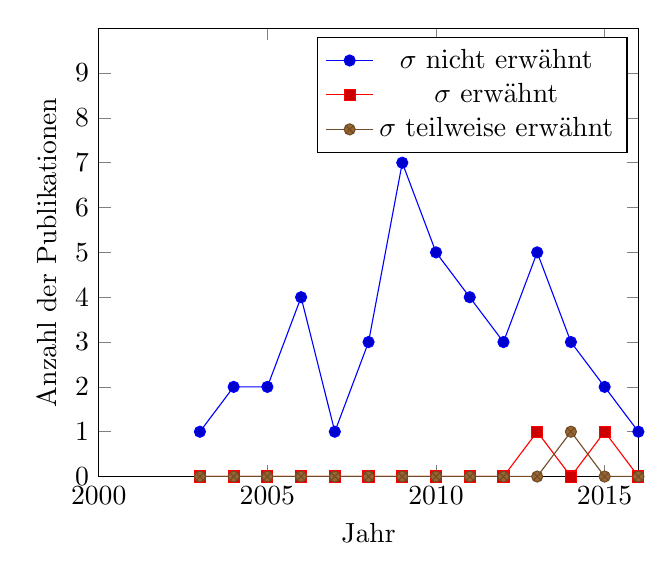
\begin{tikzpicture}
        \begin{axis}[
        ymin=0,
        ymax=10,
        %xtick = 1,
        bar shift=0pt,
        %enlarge x limits=0.10,
        xtick = {2000, 2005, 2010, 2015},
        xmin = 2000,
        xmax = 2016,
        ytick = {0, ..., 9},
        cycle list name=auto,
        %every axis plot/.append style={ybar interval, opacity=0.75,fill,draw=black,no markers},
        ylabel={Anzahl der Publikationen},
        xlabel=Jahr,
        x tick label style={/pgf/number format/.cd, set thousands separator={}},
        legend entries={$\sigma$ nicht erwähnt\\$\sigma$ erwähnt\\$\sigma$ teilweise erwähnt\\}
        ]
            \addplot coordinates {(2003, 1) (2004, 2) (2005, 2) (2006, 4) (2007, 1) (2008, 3) (2009, 7) (2010, 5) (2011, 4) (2012, 3) (2013, 5) (2014, 3) (2015, 2) (2016, 1)};
            \addplot coordinates {(2003, 0) (2004, 0) (2005, 0) (2006, 0) (2007, 0) (2008, 0) (2009, 0) (2010, 0) (2011, 0) (2012, 0) (2013, 1) (2014, 0) (2015, 1) (2016, 0)};
            \addplot coordinates {(2003, 0) (2004, 0) (2005, 0) (2006, 0) (2007, 0) (2008, 0) (2009, 0) (2010, 0) (2011, 0) (2012, 0) (2013, 0) (2014, 1) (2015, 0) (2016, 0)};
        \end{axis}
    \end{tikzpicture}

    std = 2 und   4\%, both = 1 und   2\%, no std = 43 und  93\%


    
\end{document}
        
